%
% related-work.tex
%
% Copyright (C) 2022 by Universidade Federal de Santa Catarina.
%
% GNSS Networks Based on Small Satellites
%
% This work is licensed under the Creative Commons Attribution-ShareAlike 4.0
% International License. To view a copy of this license,
% visit http://creativecommons.org/licenses/by-sa/4.0/.
%

%
% \brief Related works section.
%
% \author Gabriel Mariano Marcelino <gabriel.mm8@gmail.com>
%
% \version 0.0.0
%
% \date 2021/06/14
%

\section{Related Work} \label{sec:related-work}

\subsection{Current GNSS networks}

Atualmente existem N redes de GNSS em operação, X em fase de implantação e testes e Y redes em planejamento.

Abaixo, encontra-se uma descrição de cada uma dessas redes.

\subsubsection{GPS}

\subsubsection{GLONASS}

O GLONASS, sigla de \textit{Globalnaya navigatsionnaya sputnikovaya sistema} (ou Sistema de Navegação Global por Satélite), é o sistema de GNSS criado e mantido pela Rússia.

\subsubsection{Galileo}

O Galileo é o sistema de GNSS criado pela união europeia.

\subsubsection{BeiDou}

BeiDou, ou \textit{BeiDou Navigation Satellite System} (BDS) é o sistema de GNSS chinês.






A \autoref{tab:gnss-networks} compara as principais características dos sistemas de GNSS apresentados acima.


\cite{aarestad2020}

\begin{figure}[!ht]
    \begin{center}
        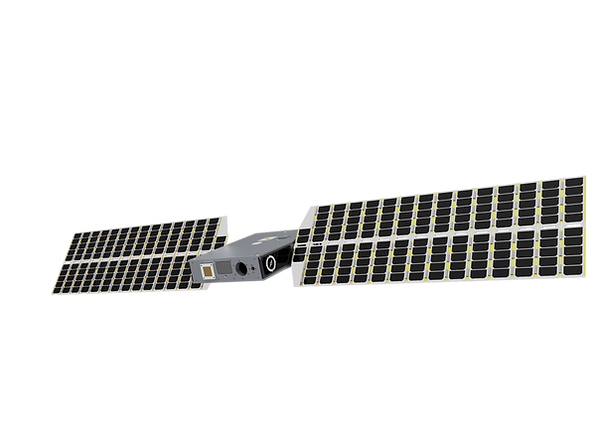
\includegraphics[width=\columnwidth]{figures/xona-satellite}
        \caption{Xona Space Systems conceptual satellite.}
        \label{fig:xona-satellite}
    \end{center}
\end{figure}

\subsection{Experimental GNSS networks}
